% =====================================================================
% ELE637 -- Pensamento Sistêmico em Engenharia
% Trabalho Prático: desvios ambientais por falha humana (DLC + ABM)
% =====================================================================
\documentclass[11pt, a4paper]{article}

\usepackage[utf8]{inputenc}
\usepackage[T1]{fontenc}
\usepackage[brazil]{babel}
\usepackage[margin=2.5cm]{geometry}
\usepackage{amsmath, amssymb}
\usepackage{graphicx}
% figuras próprias em figuras/; gráficos lidos direto de ../outputs (gerados pelos scripts do modelo)
\graphicspath{{figuras/}{../outputs/}}
\usepackage{booktabs}
\usepackage{array}
\usepackage{float}
\usepackage{xcolor}
\usepackage[authoryear, round]{natbib}
\usepackage[hidelinks]{hyperref}
\usepackage[protrusion=true, expansion=false]{microtype}
\usepackage[font=small]{caption}
\usepackage{enumitem}
\setlist{itemsep=1pt, topsep=3pt, parsep=0pt}

% ---------------------------------------------------------------------
\title{Dinâmica dos desvios ambientais por falha humana:\\
pressão operacional, supervisão e moral coletiva}
\author{%
  \small\begin{tabular}[t]{@{}c@{\hspace{2em}}c@{}}
    Rafael Campello Soares (2024017457) & Elias Daniel Moreira de Siqueira (2024022825) \\[4pt]
    Pedro Armando Oliveira Duarte (2024022710) &
    Henrique Viana Lima de Oliveira (2023066543)
  \end{tabular}\vspace{1em}\\
  {\small ELE637 -- Pensamento Sistêmico em Engenharia -- UFMG}
}
\date{}

\begin{document}
\maketitle
\begin{abstract}
Desvios ambientais causados por falha humana, como o descarte incorreto de resíduos, persistem mesmo em organizações com procedimentos bem definidos. Este trabalho parte da experiência de um dos integrantes com melhoria contínua no setor de Meio Ambiente de uma multinacional e pergunta como a pressão operacional, a supervisão e a moral coletiva determinam se a taxa de desvios converge para a ordem ou para a desordem. A situação é representada por um Diagrama de Loop Causal (DLC) com laços de reforço e de balanceamento e simulada por um modelo baseado em agentes, em que trabalhadores, sujeitos à pressão, ao contágio da desordem visível e à moral, erram com certa probabilidade, enquanto agentes corretores supervisionam seu entorno. No cenário base, a desordem se estabiliza em 16\% da área e nunca chega a zero. A moral é a alavanca de maior efeito (elevá-la de 0,50 para 0,75 reduz a desordem em 52\%), seguida pela pressão e pela facilidade de corrigir os desvios; um choque de pressão tem efeito transitório, dissipado em cerca de 45 passos. O contágio da desordem tem um limiar: até $\beta_D\approx2{,}8$ a resposta é suave e, entre 3,5 e 5, a desordem salta de 0,32 para 0,74. Por fim, a rota dos corretores só importa quando a supervisão é ampla: com 16 corretores, a rota de cobertura reduz a desordem de 0,124 para 0,097.

\medskip
\noindent\textbf{Palavras-chave:} pensamento sistêmico; diagrama de loop causal; modelo baseado em agentes; desvios ambientais; erro humano.
\end{abstract}

% =====================================================================
\section{Introdução}
% =====================================================================
Este trabalho tem origem na atuação de um dos integrantes do grupo com Melhoria Contínua aplicada ao Meio Ambiente em Produção, onde o foco era criar estruturas e procedimentos para prevenir desvios ambientais.

Os desvios variam em gravidade. Os \emph{leves} envolvem falta de organização, sujeira ou descarte incorreto de lixo comum, têm baixo impacto a curto e longo prazo e muitas vezes são negligenciados na prática. Os \emph{médios} exigem planos de contingência e ações corretivas para evitar recorrência, pois têm impacto significativo para o meio ambiente. Os \emph{graves}, como vazamentos de produtos químicos e emissões atmosféricas, geram multas, impacto ambiental severo e irreversível, repercussão social e risco de embargo das operações. A situação importa para a organização porque os desvios leves são frequentes e, como sugere a literatura sobre a normalização do desvio \citep{banja2010}, podem criar um ambiente em que desvios mais sérios passam a ser tolerados.

O trabalho aplica o pensamento sistêmico \citep{meadows2022,sterman2000} e a modelagem de sistemas complexos \citep{sayama2015}: do problema ao diagrama, do diagrama ao modelo computacional e do modelo à análise. A Seção~\ref{sec:situacao} descreve a situação; a Seção~\ref{sec:dlc} apresenta o modelo conceitual (DLC); a Seção~\ref{sec:modelo} define o modelo computacional; a Seção~\ref{sec:resultados} reporta e discute os resultados; e a Seção~\ref{sec:conclusao} apresenta as conclusões e recomendações.

% =====================================================================
\section{A situação estudada}\label{sec:situacao}
% =====================================================================

\subsection{Tema, horizonte de tempo e comportamento observado}\label{sec:comportamento}
O tema é a ocorrência recorrente de desvios ambientais por falha humana, tomando como caso representativo o descarte incorreto de resíduos em uma área operacional. O horizonte de interesse é de meses de operação contínua. O comportamento observado é crônico: os erros ocorrem continuamente, ora mais, ora menos, e nunca desaparecem. Há picos nos períodos de maior produção, queda depois de campanhas e ações corretivas e, em seguida, retorno gradual ao nível anterior.

\subsection{Pergunta a responder}
Existe uma dissincronia entre a empresa teórica, em que os processos são perfeitos e as pessoas seguem as regras sem errar, e a empresa real, em que os erros ocorrem o tempo todo. Embora a engenharia trate o erro como falha sistêmica, na ponta ele é executado por indivíduos. A pergunta do grupo é:
\begin{quote}
\emph{Como a pressão operacional, a supervisão e a moral coletiva interagem para determinar se os desvios ambientais por falha humana se estabilizam em um nível baixo ou se escalam para a desordem, e quais alavancas reduzem a probabilidade do erro?}
\end{quote}

\subsection{Fronteira do sistema}
\begin{itemize}
  \item \textbf{Dentro:} trabalhadores da ponta, a supervisão exercida pela empresa (medidas administrativas e orientação em campo), a pressão operacional, a moral coletiva, a desordem visível no ambiente de trabalho e o prejuízo para a empresa.
  \item \textbf{Externo (entra como entrada):} fatores externos que modulam a pressão, como demanda e prazos de produção.
  \item \textbf{Fora:} legislação e fiscalização externas, falhas de equipamento e de processo, e desvios que não dependem de decisão humana.
\end{itemize}

\subsection{A situação vista como sistema}
As partes são os trabalhadores, os supervisores, os resíduos e o ambiente físico; as relações são a influência da pressão sobre as decisões, o efeito da desordem visível sobre quem a observa e a reação da empresa aos prejuízos; o propósito é produzir mantendo a conformidade ambiental. Sinais de complexidade:
\begin{itemize}
  \item \textbf{Laços que se reforçam e que competem:} a desordem visível induz mais desordem, enquanto a supervisão e a moral a combatem (Seção~\ref{sec:dlc}).
  \item \textbf{Atrasos:} entre o prejuízo e a reação administrativa, e entre as medidas sociais e a moral.
  \item \textbf{Efeito contraintuitivo e resistência a políticas:} medidas administrativas que, ao pressionar a operação, podem aumentar o erro que pretendiam reduzir.
  \item \textbf{Não linearidade e limiar:} o efeito da desordem sobre o comportamento é pequeno até certo ponto e depois cresce rapidamente; acima de certo nível a norma de não descartar de forma incorreta pode colapsar, como em estudos sobre descarte de lixo \citep{rangoni2017}.
  \item \textbf{Emergência:} padrões globais de ordem ou desordem surgem de interações locais entre vizinhos.
\end{itemize}

Segundo o relato do integrante, há três causas-raiz da falha humana, ilustradas no descarte incorreto:
\begin{enumerate}
  \item \textbf{Pressão operacional (falta de tempo e sobrecarga):} quando o ritmo aperta, o colaborador prioriza a produção e dedica menos tempo a pensar no descarte correto, e deixa o resíduo no local mais próximo.
  \item \textbf{Complexidade e esquecimento (sobrecarga cognitiva):} a variedade de insumos usados diariamente (centenas de tipos de tintas, lixas, graxas e produtos químicos) gera dúvida sobre a destinação correta e leva a descartes aleatórios.
  \item \textbf{Desengajamento (negligência):} mesmo sem pressão e conhecendo a regra, há pessoas que erram por não se importarem com o meio ambiente ou com as consequências coletivas.
\end{enumerate}

% =====================================================================
\section{Modelo conceitual}\label{sec:dlc}
% =====================================================================
A Figura~\ref{fig:dlc} apresenta o DLC. O nó central é o \emph{desvio operacional humano}, que na Seção~\ref{sec:modelo} é tratado como a probabilidade de um trabalhador errar. Quatro variáveis agem diretamente sobre ele (pressão, desordem visível, medidas administrativas e medida social); a moral age por meio da desordem visível; e o próprio desvio realimenta o sistema por dois caminhos, a desordem visível e o prejuízo para a empresa.

\begin{figure}[H]
  \centering
  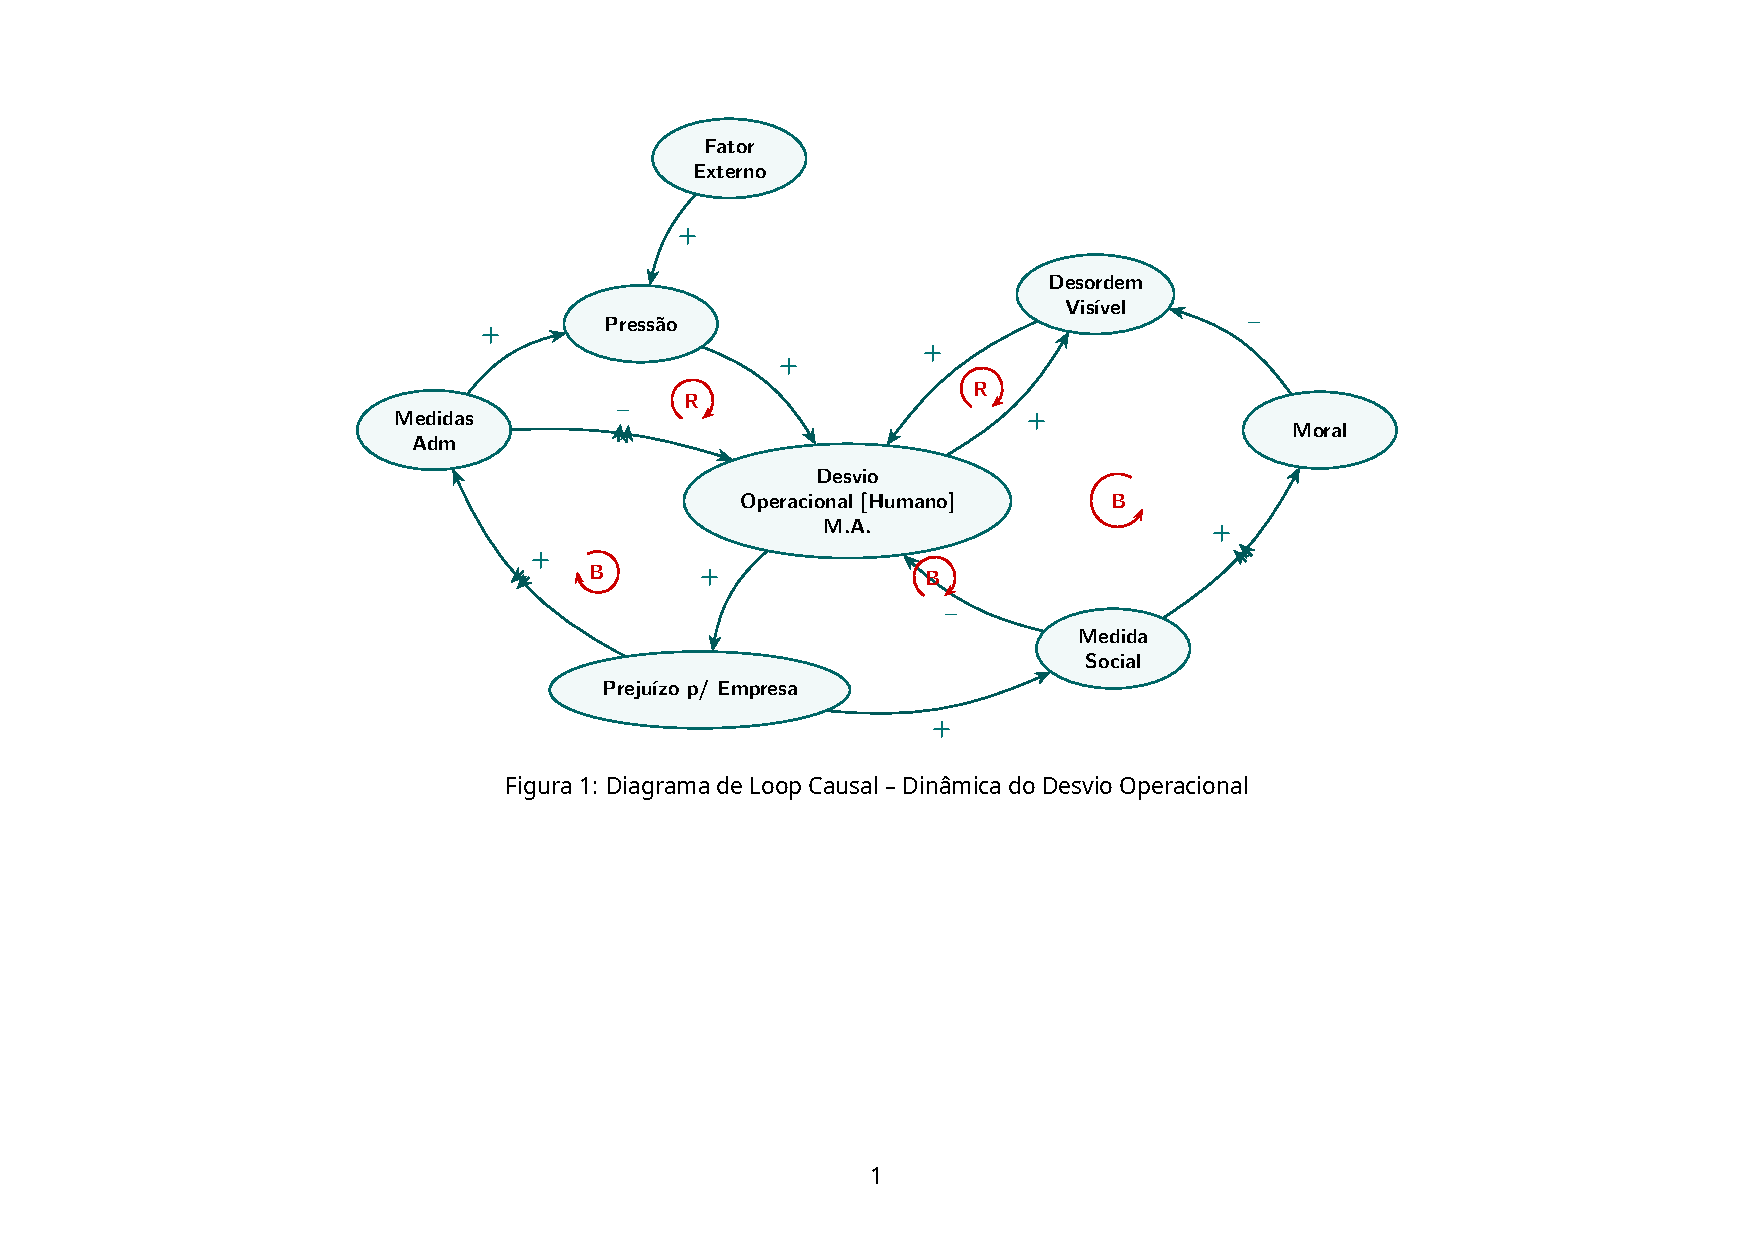
\includegraphics[trim=160pt 235pt 160pt 50pt, clip, width=0.6\textwidth]{figuras/diagrama_loop_causal.pdf}
  \caption{Diagrama de Loop Causal da dinâmica do desvio operacional. Os laços R são de reforço e os laços B de balanceamento. Os traços duplos nas setas indicam atrasos.}
  \label{fig:dlc}
\end{figure}

\paragraph{Exemplo de referência.}
Considere o trabalhador médio (moral $M=0{,}5$) em um turno de pressão intermediária ($P=0{,}5$), sem resíduos à vista ($D=0$) e sem supervisor por perto ($S=0$). Pela regra do modelo (Seção~\ref{sec:modelo}), a probabilidade de descartar incorretamente um resíduo em uma hora de trabalho é $\sigma(-2{,}4)=8{,}3\%$, ou seja, um erro a cada 12 horas por pessoa e cerca de 10 erros por hora em uma equipe de 120 trabalhadores. Cada laço do DLC altera esse número de uma forma específica, como mostram os exemplos a seguir e a Tabela~\ref{tab:lacos}.

\paragraph{Laços de reforço.}
\begin{itemize}
  \item \textbf{R1 (desordem visível):} desvio $\rightarrow$ desordem visível $\rightarrow$ mais desvio. É o contágio em que ver erros por perto torna o erro mais provável, o mecanismo associado à teoria das janelas quebradas \citep{ball2012}. \emph{Exemplo:} um operador que encontra quatro das oito células vizinhas com resíduos ($D=0{,}5$) passa de 8,3\% para 15,4\% de probabilidade de errar (1,9 vez mais); se a vizinhança inteira está suja ($D=1$), a probabilidade chega a 26,9\% (3,2 vezes).
  \item \textbf{R2 (resistência a políticas):} desvio $\rightarrow$ prejuízo $\rightarrow$ medidas administrativas $\rightarrow$ pressão $\rightarrow$ mais desvio. A reação da empresa, quando aumenta a pressão sobre a operação, realimenta o problema que pretendia resolver. \emph{Exemplo:} uma cobrança de metas ou uma auditoria que eleve $P$ de 0,5 para 1,0 aumenta a probabilidade de erro de 8,3\% para 14,2\% (1,7 vez), enquanto uma operação sem pressão ($P=0$) teria 4,7\%.
\end{itemize}

\paragraph{Laços de balanceamento.}
\begin{itemize}
  \item \textbf{B1 (supervisão):} desvio $\rightarrow$ prejuízo $\rightarrow$ medidas administrativas $\rightarrow$ menos desvio, com atraso entre o prejuízo e a reação. \emph{Exemplo:} a presença de um supervisor em um raio de três células ($S=1$) reduz a probabilidade de erro do trabalhador de 8,3\% para 3,2\% (61\% menos), efeito consistente com o ganho de conformidade sob observação relatado na literatura \citep{srigley2014}.
  \item \textbf{B2 (medida social):} desvio $\rightarrow$ prejuízo $\rightarrow$ medida social $\rightarrow$ menos desvio. É o efeito \emph{imediato} da correção feita por um funcionário da empresa que encontra o resíduo, o remove e dá \emph{feedback} ao responsável no próprio local. \emph{Exemplo:} um agente de campo que passa pela célula suja a limpa com probabilidade de 88\% por passo, contra 50\% para o trabalhador médio.
  \item \textbf{B3 (moral):} desvio $\rightarrow$ prejuízo $\rightarrow$ medida social $\rightarrow$ moral $\rightarrow$ menos desordem visível $\rightarrow$ menos desvio, com atraso na formação da moral. As medidas sociais aqui são as palestras, treinamentos e eventos da empresa, cujo efeito se acumula lentamente. \emph{Exemplo:} elevar a moral média de 0,50 para 0,75 reduz a probabilidade de erro de 8,3\% para 5,2\% (37\% menos) e eleva a probabilidade de corrigir um resíduo de 50\% para 68\%.
\end{itemize}

\begin{table}[t]
\centering
\footnotesize
\caption{Laços do DLC, exemplo concreto e efeito na probabilidade de erro do trabalhador médio (8,3\% na referência $P=0{,}5$, $M=0{,}5$, $D=0$, $S=0$). Os valores resultam das equações da Seção~\ref{sec:modelo}.}
\label{tab:lacos}
\begin{tabular}{@{}llp{5.2cm}l@{}}
\toprule
Laço & Tipo & Exemplo na área operacional & Efeito quantificado \\
\midrule
R1 & Reforço & Resíduo visível nas células vizinhas & $D=0{,}5$: 15,4\%; $D=1$: 26,9\% \\
R2 & Reforço & Cobrança de metas após um prejuízo & $P=1$: 14,2\%; $P=0$: 4,7\% \\
B1 & Balanceamento & Supervisor presente no entorno & $S=1$: 3,2\% \\
B2 & Balanceamento & Correção imediata e \emph{feedback} no local & Remoção do resíduo: 88\% (agente) \\
B3 & Balanceamento & Palestras e eventos que elevam a moral & $M=0{,}75$: 5,2\%; $M=0{,}25$: 13,0\% \\
\bottomrule
\end{tabular}
\end{table}

O fator externo entra apenas como entrada que aumenta a pressão. O par B1--R2 corresponde ao arquétipo \emph{soluções que falham} \citep{meadows2022}: a medida administrativa reduz o desvio, mas só depois de um atraso, enquanto a pressão que ela gera age de imediato e realimenta o problema. Por isso as melhoras obtidas por medidas administrativas tendem a ser temporárias, como no comportamento descrito na Seção~\ref{sec:comportamento}.

% =====================================================================
\section{Modelo computacional}\label{sec:modelo}
% =====================================================================
\subsection{Delimitação temporal e simplificações do modelo}
O modelo computacional representa uma aproximação de curto prazo da dinâmica do DLC. Um passo de tempo corresponde a cerca de uma hora de operação, e uma execução de 600 passos cobre algumas semanas de turnos. Nessa escala, os laços que dependem de atrasos organizacionais (a implementação de medidas administrativas, em R2 e B1, e a formação gradual da moral, em B3) são lentos demais para variar dentro de uma execução. Por isso a pressão operacional e a moral são tratadas como parâmetros exógenos, constantes em cada execução, e o efeito desses laços é estudado comparando execuções com valores diferentes de $P$ e $\bar M$. A desordem visível e a posição dos corretores mudam a cada passo, de modo que o laço R1, a correção e a supervisão em campo são representados diretamente. Uma versão futura poderá tornar $P$ e $M$ variáveis no tempo, com os atrasos do DLC.

Foi escolhido um \textbf{modelo baseado em agentes sobre uma grade}, com regras locais de vizinhança no estilo de um autômato celular. A escolha se justifica porque (i) o fenômeno emerge de interações locais, já que o erro de um trabalhador afeta quem está por perto; (ii) trabalhadores e corretores se movem, de modo que a posição importa; e (iii) a moral varia de pessoa para pessoa, o que um modelo de estoque e fluxo não representaria sem um estoque para cada nível de moral. Modelos semelhantes foram usados para estudar o descarte de lixo e o colapso de normas \citep{rangoni2017} e o papel de agentes que fazem normas valerem \citep{savarimuthu2008}.

\subsection{Agentes e ambiente}
\begin{itemize}
  \item \textbf{Ambiente:} grade $L\times L$ com fronteira toroidal. Cada célula pode conter resíduo descartado incorretamente, o que representa a desordem visível.
  \item \textbf{Trabalhadores ($N_T$):} agentes móveis. A cada passo, cada trabalhador $i$ descarta um resíduo de forma incorreta com probabilidade $pdt_i(t)$ e corrige o resíduo da sua célula com probabilidade $pct_i$.
  \item \textbf{Corretores ($K$):} agentes móveis que representam a supervisão em campo. Reduzem o erro dos trabalhadores a até $r_s$ células de distância, erram com probabilidade $pda_i(t)$ e corrigem com probabilidade $pca_i$.
\end{itemize}
Cada célula comporta no máximo um agente, mas um resíduo pode estar na célula de um agente.

\subsection{Regras do modelo}
\paragraph{Moral individual.}
A pressão operacional $P\in[0,1]$ é comum a todos. A moral, ao contrário, é heterogênea e fixa para cada agente $i$:
\[
M_i \sim \mathrm{clip}\!\left(\mathcal{N}(\bar{M},\sigma_M^2),\,0,\,1\right),
\]
em que $\bar{M}$ é a moral média da equipe e $\sigma_M$ mede a dispersão entre os agentes. Valores baixos de $M_i$ representam trabalhadores desengajados (causa-raiz 3), que erram mesmo sem pressão e raramente corrigem desvios.

\paragraph{Probabilidade de erro.}
Para trabalhadores e corretores, respectivamente,
\begin{align*}
pdt_i(t)&=\sigma\!\left(b_T+\beta_P^T P+\beta_D^T D_i(t)-\beta_S^T S_i(t)-\beta_M^T M_i\right),\\
pda_i(t)&=\sigma\!\left(b_A+\beta_P^A P+\beta_D^A D_i(t)-\beta_M^A M_i\right),
\end{align*}
em que $\sigma(x)=1/(1+e^{-x})$ é a função logística. Os interceptos $b_T>b_A$ representam a propensão basal ao erro (causa-raiz 2), maior para quem lida diretamente com os insumos. Os coeficientes $\beta$ são positivos; o corretor não sofre efeito da supervisão.

\paragraph{Probabilidade de correção.}
Um agente remove o resíduo da sua célula com probabilidade
\[
pct_i=\sigma\!\left(c_T+\gamma_M^T M_i\right)
\quad\text{(trabalhadores)},
\qquad
pca_i=\sigma\!\left(c_A+\gamma_M^A M_i\right)
\quad\text{(corretores)}.
\]

\paragraph{Desordem local e supervisão.}
A desordem percebida é a fração das 8 células da vizinhança de Moore (sem a própria) com resíduo, $D_i(t)=\frac{1}{8}\sum_{j\in\mathcal{R}_i}X_j(t)$, com $X_j(t)\in\{0,1\}$. A supervisão $S_i(t)$ vale 1 se há ao menos um corretor a distância de Chebyshev $\le r_s$, e 0 caso contrário.

\paragraph{Ordem de execução em cada passo.}
A Tabela~\ref{tab:ordem} resume as quatro etapas. As etapas 1 a 3 usam o estado do início do passo e não dependem da ordem dos agentes; o movimento é sequencial porque cada deslocamento altera as células livres.

\begin{table}[t]
\centering
\footnotesize
\caption{Etapas executadas em cada passo de tempo.}
\label{tab:ordem}
\begin{tabular}{@{}clp{8.2cm}@{}}
\toprule
Etapa & Nome & Operação \\
\midrule
1 & Percepção & Cada agente calcula $D_i(t)$ e $S_i(t)$ com o estado da grade no início do passo. \\
2 & Erro & Com probabilidade $pdt_i$ (ou $pda_i$), o agente descarta um resíduo na célula em que está; descartes corretos não deixam marca na grade. \\
3 & Correção & Se havia resíduo na célula no início do passo, o agente o remove com probabilidade $pct_i$ (ou $pca_i$); se erra e corrige no mesmo passo, o erro prevalece. \\
4 & Movimento & Em ordem aleatória sorteada a cada passo, cada agente vai para uma célula vizinha livre ou permanece onde está, conforme sua política. \\
\bottomrule
\end{tabular}
\end{table}

\paragraph{Políticas de movimento.}
Os trabalhadores andam ao acaso. Cada corretor avalia a própria célula e as vizinhas livres (até nove candidatas), atribui uma pontuação a cada uma e vai para a de maior pontuação, com desempate ao acaso; com probabilidade $\varepsilon$ ignora a pontuação e anda ao acaso. Foram definidas três políticas (Tabela~\ref{tab:politicas}).
Por exemplo, com $r_s=3$ a política reativa compara janelas de $7\times7=49$ células: se a candidata A tem 6 resíduos na janela e a candidata B tem 2, o corretor vai para A; na política de cobertura, a candidata mais distante do corretor mais próximo vence. Na reativa, a supervisão forma um laço de balanceamento com a desordem; nas outras duas, ela é uma influência sem realimentação.

\begin{table}[t]
\centering
\footnotesize
\caption{Políticas de movimento dos corretores.}
\label{tab:politicas}
\begin{tabular}{@{}lp{4.3cm}p{4.2cm}l@{}}
\toprule
Política & Pontuação da célula candidata & Intenção & Realimentação \\
\midrule
Aleatória & Igual para todas & Supervisão sem informação (cenário base) & Não \\
Reativa & Nº de células com resíduo a distância $\le r_s$ & Concentrar a supervisão onde o problema já apareceu & Sim \\
De cobertura & Distância de Chebyshev ao corretor mais próximo & Espalhar a supervisão pela área antes que haja desordem & Não \\
\bottomrule
\end{tabular}
\end{table}

\begin{table}[t]
\centering
\footnotesize
\caption{Parâmetros do modelo, valores base, faixas testadas e evidência que sustenta a escolha.}
\label{tab:parametros_modelo}
\begin{tabular}{@{}lllp{7.6cm}@{}}
\toprule
Símbolo & Base & Faixa & Ancoragem \\
\midrule
$L$; $N_T$, $K$ & 30; 120, 8 & $K\in[0,16]$ & 14\% das células ocupadas por agentes \\
$r_s$ & 3 & 1--5 & alcance visual em campo (escolha de modelagem) \\
$P$ & 0,5 & $[0,1]$ & varredura completa \\
$\bar{M}$, $\sigma_M$ & 0,5; 0,25 & $\bar M\in[0,1]$ & dispersão alta, como em \citet{rangoni2017} \\
$b_T$, $b_A$ & $-2{,}0$; $-3{,}0$ & --- & erro basal de 2--10\% em tarefas rotineiras \citep{kirwan1994} \\
$\beta_P^T$, $\beta_P^A$ & 1,2; 0,6 & --- & efeito pequeno a moderado da pressão \citep{szalma2008} \\
$\beta_D^T$, $\beta_D^A$ & 1,4; 1,4 & 0--8 & ambiente desordenado dobra o descarte indevido \citep{keizer2008,cialdini1990} \\
$\beta_S^T$ & 1,0 & 0--2 & observador visível triplica a conformidade \citep{srigley2014} \\
$\beta_M^T$, $\beta_M^A$ & 2,0; 2,0 & --- & clima de segurança prediz conformidade \citep{christian2009} \\
$c_T$, $c_A$ & $-1{,}5$; $1{,}0$ & $c_T\in[-3,0]$ & corretores têm papel explícito de limpeza \citep{rangoni2017} \\
$\gamma_M^T$, $\gamma_M^A$ & 3,0; 2,0 & --- & com $M=0{,}5$: $pct=0{,}5$ e $pca=0{,}88$ \\
$\varepsilon$ & 0,1 & --- & ruído no movimento, como em \citet{rangoni2017} \\
$T$ & 600 & --- & regime estacionário em menos de 100 passos \\
\bottomrule
\end{tabular}
\end{table}

\subsection{Protocolo experimental}
O modelo foi implementado em Python (NumPy 2.5 e Matplotlib 3.11). Cada configuração é simulada a partir de uma grade limpa, com sementes aleatórias distintas, e a variável de resposta é a \emph{desordem final}: a média da fração de células com resíduo nos últimos 50 dos 600 passos. As médias são relatadas com intervalo de confiança de 95\% (distribuição $t$ de Student) sobre as sementes. O cenário base, a comparação entre alavancas e as políticas de movimento usam 20 sementes por configuração; as varreduras de sensibilidade e a tabela $P\times K$ usam 10; as curvas das Figuras~\ref{fig:base} e~\ref{fig:extremos} usam 10 e 5 sementes, respectivamente, e os tempos de convergência e de recuperação do choque citados no texto foram medidos em 10 sementes independentes; a varredura do contágio usa 4. Como os parâmetros vêm da literatura e não foram calibrados, os valores absolutos de desordem têm caráter ilustrativo, e a análise se concentra em comparações relativas entre configurações.

% =====================================================================
\section{Resultados e discussão}\label{sec:resultados}
% =====================================================================

\subsection{Cenário base}
A Figura~\ref{fig:base} mostra a evolução da fração de células com resíduo (desordem) e da taxa de erro dos trabalhadores a partir de uma grade limpa, e o estado final de uma execução. A desordem atinge metade do patamar em cerca de 11 passos e 90\% dele em cerca de 45 passos, e depois oscila em torno de 0,160 (IC 95\%: $\pm0{,}009$; desvio-padrão entre sementes de 0,018), isto é, cerca de 144 das 900 células. A taxa de erro dos trabalhadores fica em 9,1\%, ou seja, cerca de 11 descartes incorretos por passo na equipe de 120. O estado final mostra que os resíduos se agrupam em manchas, o sinal do contágio local (R1), e que os oito corretores cobrem apenas parte da área.

\textbf{Conclusão:} os desvios não desaparecem, não crescem sem limite e se estabilizam em torno de um nível único, o mesmo padrão qualitativo observado na área (Seção~\ref{sec:comportamento}). O nível absoluto não foi comparado com dados reais.

\begin{figure}[tbp]
  \centering
  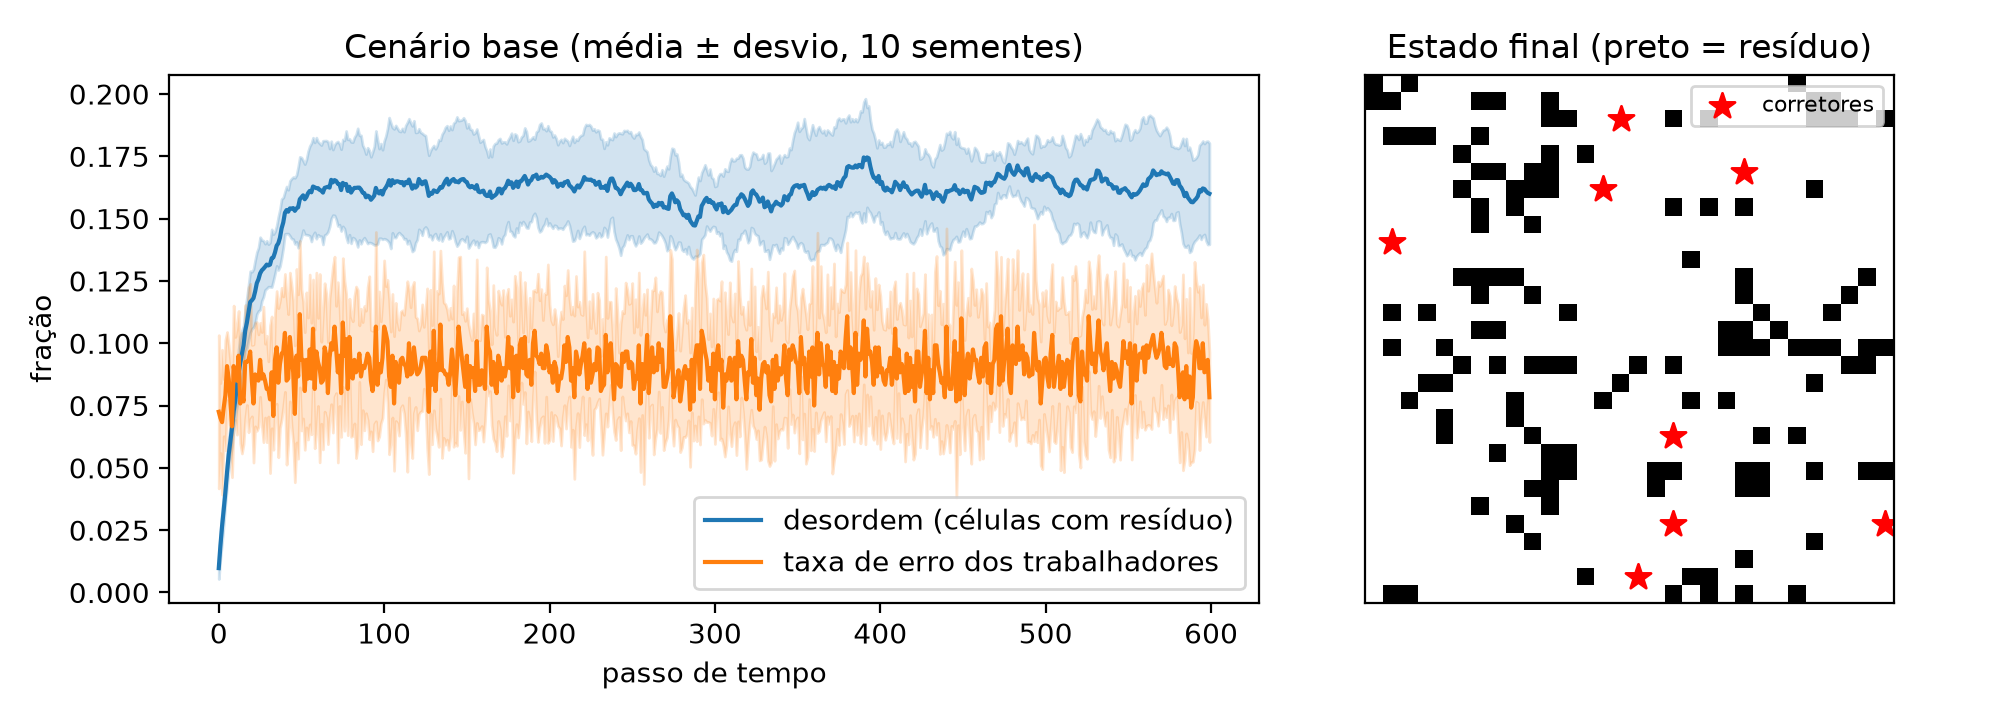
\includegraphics[width=0.85\textwidth]{fig1_cenario_base.png}
  \caption{Cenário base: desordem e taxa de erro dos trabalhadores (média $\pm$ desvio de 10 sementes) e estado final da grade (preto: resíduo; estrelas: corretores).}
  \label{fig:base}
\end{figure}

\subsection{Valores extremos e resposta a um choque de pressão}
A Figura~\ref{fig:extremos} (esquerda) leva um parâmetro por vez ao extremo e a Figura~\ref{fig:extremos} (direita) aplica um choque de pressão. Todos os casos extremos convergem para um patamar estável em 50 a 150 passos. Em relação ao cenário base (0,16), a desordem final fica em 0,03 com moral máxima ($-81\%$), 0,09 com pressão nula ($-44\%$), 0,22 sem corretores ($+38\%$), 0,28 com pressão máxima ($+75\%$) e 0,64 com moral nula (quatro vezes o valor base). A amplitude de cada parâmetro (diferença entre seus extremos) é 0,61 para a moral, 0,19 para a pressão e 0,06 para a presença de corretores. A moral é o parâmetro de maior efeito porque age duas vezes: reduz o erro e aumenta a correção.

No choque, a pressão sobe para $P=1$ entre os passos 100 e 150. A desordem sobe de 0,16 para 0,27 (+0,11, ou +67\%) ao fim do choque, valor próximo ao patamar de uma operação com $P=1$ permanente (0,28), de modo que 50 passos bastam para quase atingir o novo equilíbrio. Depois que a pressão volta a 0,5, o excesso de desordem cai de 0,10 para 0,06, 0,03 e 0,01 após 10, 20 e 40 passos, o que corresponde a uma meia-vida de cerca de 10 passos, e a série volta a ficar a menos de 0,01 do cenário sem choque em cerca de 45 passos. Não há efeito permanente.

\textbf{Conclusão:} o equilíbrio do sistema é estável e pouco sensível à história da operação; picos de pressão geram danos transitórios, mas a moral da equipe e a correção determinam o nível em que ele repousa.

\begin{figure}[tbp]
  \centering
  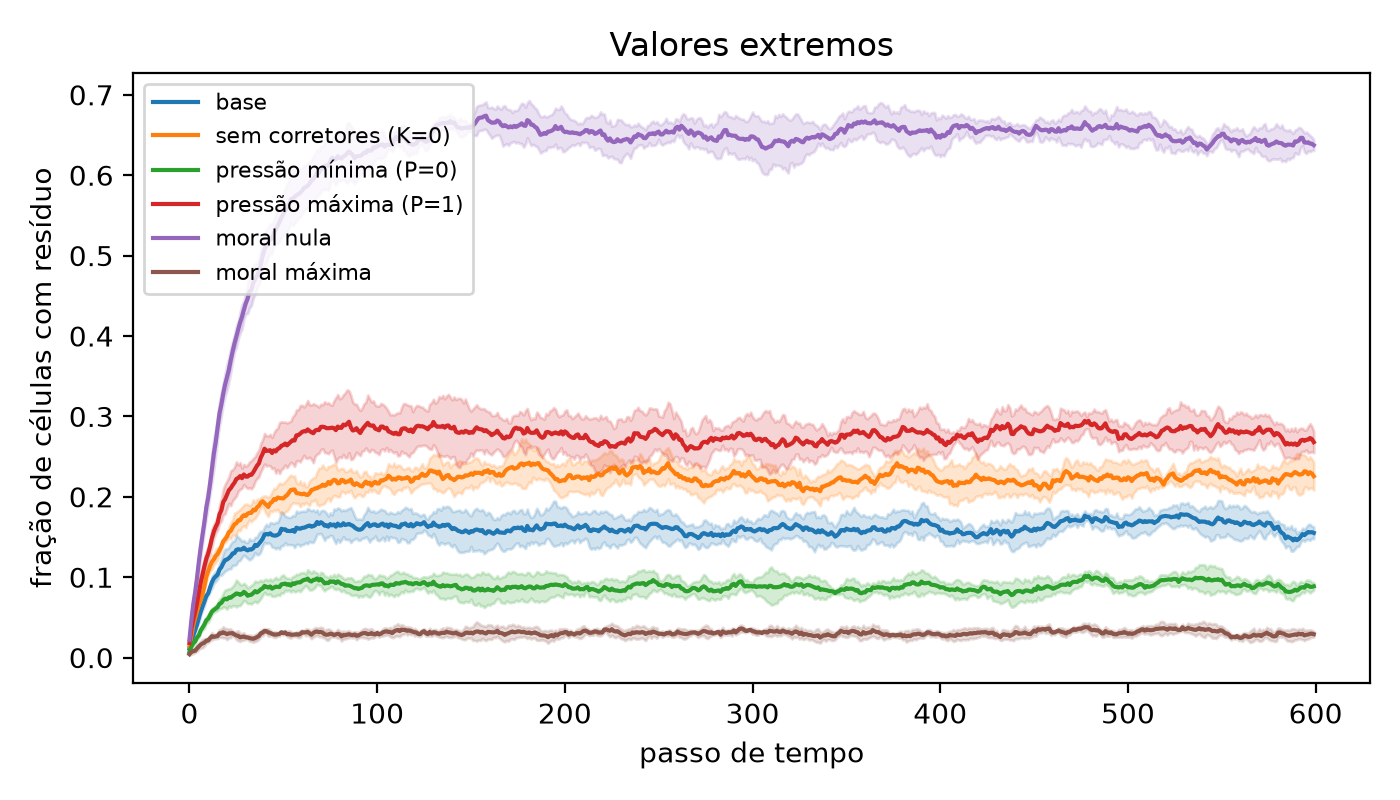
\includegraphics[width=0.49\textwidth]{fig2_extremos.png}\hfill
  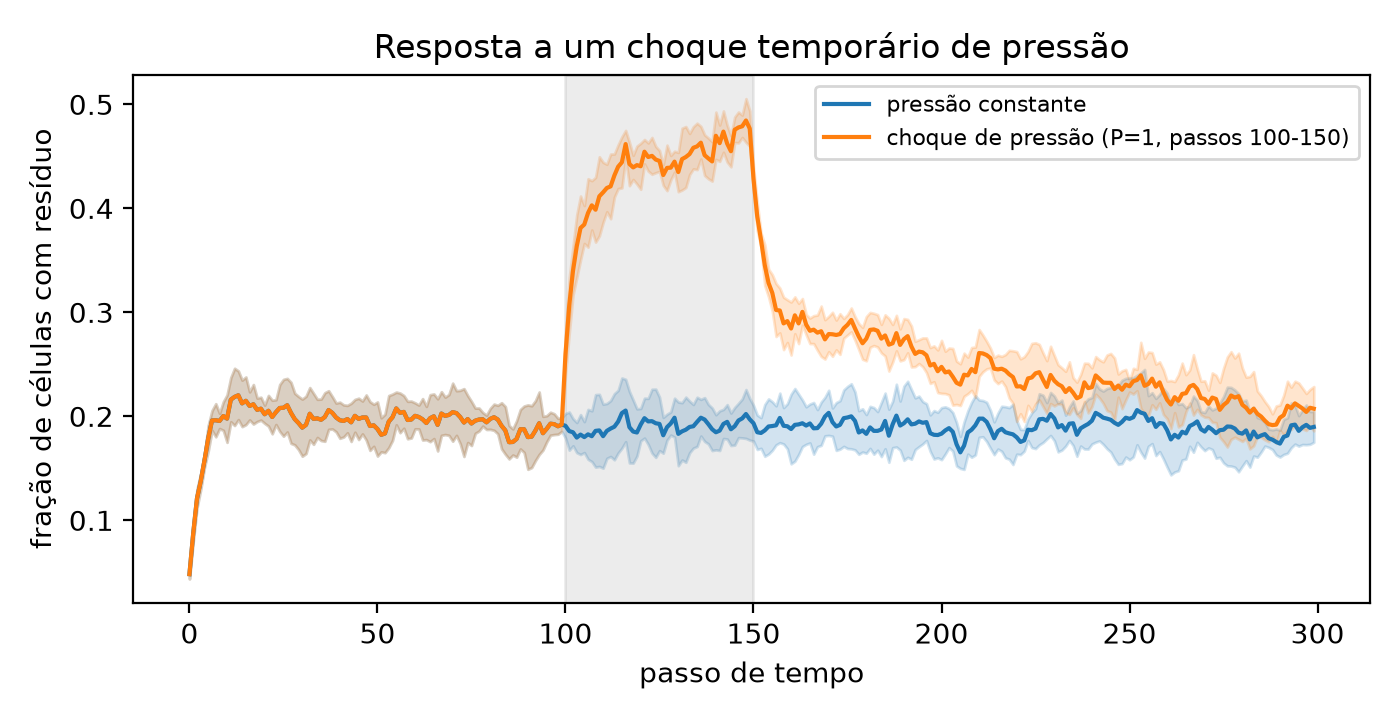
\includegraphics[width=0.49\textwidth]{fig5_choque_pressao.png}
  \caption{Esquerda: desordem ao longo do tempo para valores extremos de $K$, $P$ e $\bar M$ (média $\pm$ desvio de 5 sementes). Direita: resposta a um choque temporário de pressão ($P=1$ nos passos 100 a 150, faixa cinza).}
  \label{fig:extremos}
\end{figure}

\subsection{Pressão operacional e número de corretores}
A Tabela~\ref{tab:PK} cruza a pressão com o número de corretores. A desordem varia de forma gradual, de 0,069 ($P=0$, $K=16$) a 0,372 ($P=1$, $K=0$). Sem corretores, passar de $P=0$ para $P=1$ multiplica a desordem por 3,1 (0,120 para 0,372). Os primeiros oito corretores reduzem a desordem em 24\% a 26\% em qualquer nível de pressão, mas o ganho absoluto é maior quando a pressão é alta: 0,095 com $P=1$ contra 0,029 com $P=0$. Os corretores compensam apenas parte da pressão: com 16 corretores e pressão máxima, a desordem (0,215) é 34\% maior que a do cenário base e equivale à de uma operação sem corretores com pressão média (0,221).

\textbf{Conclusão:} a supervisão atenua a pressão, mas não a substitui; reduzir a causa (a pressão) é mais eficaz que ampliar a equipe de supervisão.

\begin{table}[t]
\centering
\footnotesize
\caption{Desordem final em função da pressão $P$ e do número de corretores $K$ (média de 10 sementes; IC 95\% de $\pm0{,}005$ a $\pm0{,}020$).}
\label{tab:PK}
\begin{tabular}{@{}cccc@{}}
\toprule
 & $K=0$ & $K=8$ & $K=16$ \\
\midrule
$P=0$ & 0,120 & 0,091 & 0,069 \\
$P=0{,}5$ & 0,221 & 0,163 & 0,126 \\
$P=1$ & 0,372 & 0,277 & 0,215 \\
\bottomrule
\end{tabular}
\end{table}

\subsection{Contágio da desordem e limiar}
A Figura~\ref{fig:limiar} varia o peso do contágio $\beta_D$ partindo de uma grade limpa e de uma grade 70\% suja, para verificar se há dois equilíbrios (histerese). As duas curvas coincidem: existe um único equilíbrio para cada valor de $\beta_D$. A resposta, porém, é fortemente não linear. Até $\beta_D=2{,}8$ a desordem sobe de 0,131 para 0,234, cerca de 0,04 por unidade de $\beta_D$. Entre 4 e 5 ela sobe de 0,424 para 0,743, cerca de 0,32 por unidade, nove vezes mais depressa; em $\beta_D=6$ chega a 0,945 e em $\beta_D=8$ a 0,995, praticamente toda a área. No cenário base ($\beta_D=1{,}4$) o contágio responde por apenas 0,029 dos 0,160 (18\%), e seria preciso mais que dobrar $\beta_D$ (de 1,4 para 3,5) para duplicar a desordem (de 0,16 para 0,32).

\textbf{Conclusão:} o limiar do laço R1 está na faixa $\beta_D\approx3$ a 5. Abaixo dele o contágio é um agravante moderado, acima dele a norma de descarte correto colapsa, e a margem de segurança do cenário base é grande.

\begin{figure}[tbp]
  \centering
  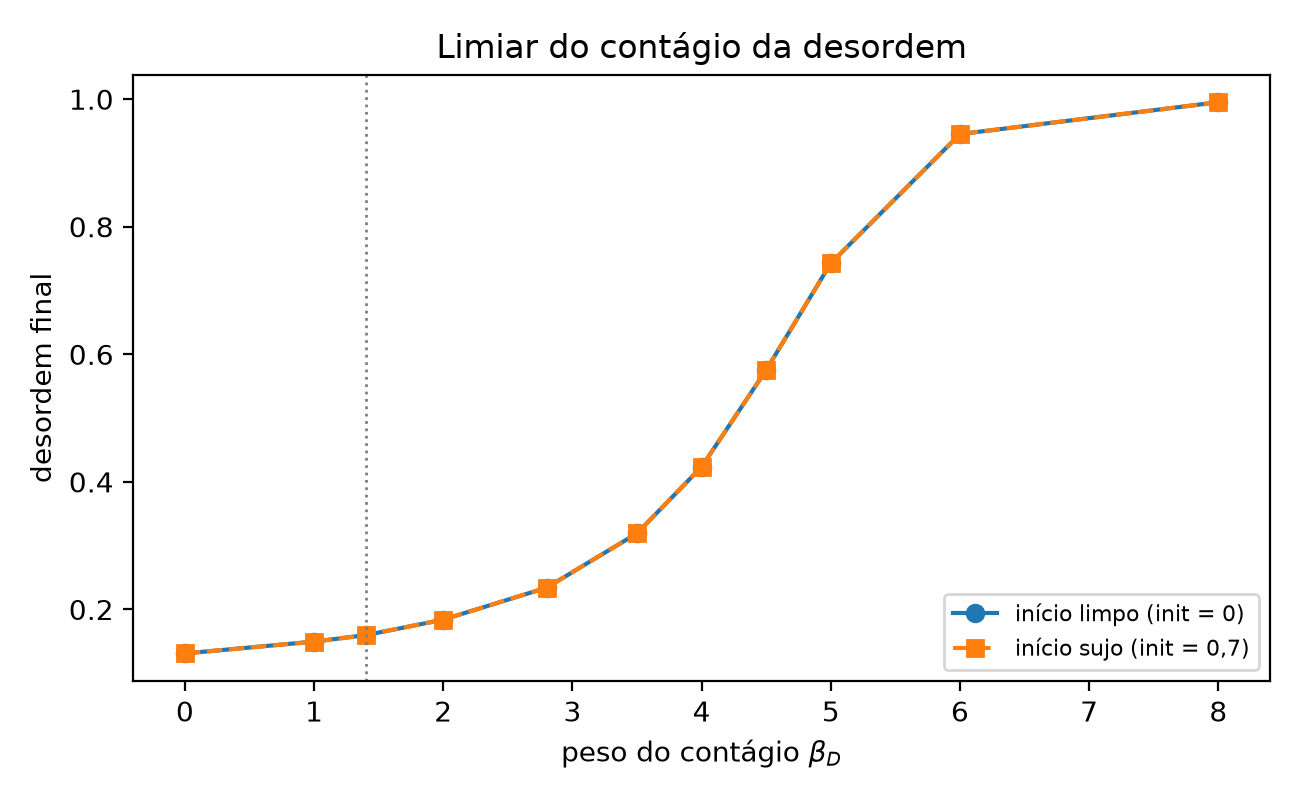
\includegraphics[width=0.6\textwidth]{fig6_limiar_contagio.png}
  \caption{Desordem final em função do peso do contágio $\beta_D$, com início limpo e início sujo (as curvas se sobrepõem); a linha pontilhada marca o valor base.}
  \label{fig:limiar}
\end{figure}

\subsection{Sensibilidade dos parâmetros incertos}
A Figura~\ref{fig:sens} varia, um de cada vez, os quatro parâmetros mais incertos (política aleatória, 10 sementes; a linha pontilhada marca o cenário base, 0,160). A correção basal dos trabalhadores $c_T$ tem o maior efeito: a desordem cai de 0,338 para 0,103 ($-70\%$) quando $c_T$ vai de $-3$ a 0, com retornos decrescentes (cada passo de 0,75 reduz 0,107 no início da faixa e 0,021 no fim). O peso do contágio $\beta_D$ eleva a desordem de 0,132 para 0,237 entre 0 e 2,8. O raio de supervisão $r_s$ reduz a desordem de 0,200 para 0,121 ($-40\%$) quando vai de 1 a 5, cerca de 0,02 por unidade. O peso da supervisão $\beta_S$ tem o menor efeito (0,206 para 0,146, $-29\%$) e satura: de 0 a 1 a queda é de 0,043, e de 1 a 2 é de 0,017. Em ordem de amplitude, $c_T$ (0,235) supera $\beta_D$ (0,105), $r_s$ (0,079) e $\beta_S$ (0,060).

\textbf{Conclusão:} a facilidade de corrigir o desvio é o parâmetro incerto que mais importa; ampliar o alcance da supervisão rende mais que torná-la mais intensa.

\begin{figure}[tbp]
  \centering
  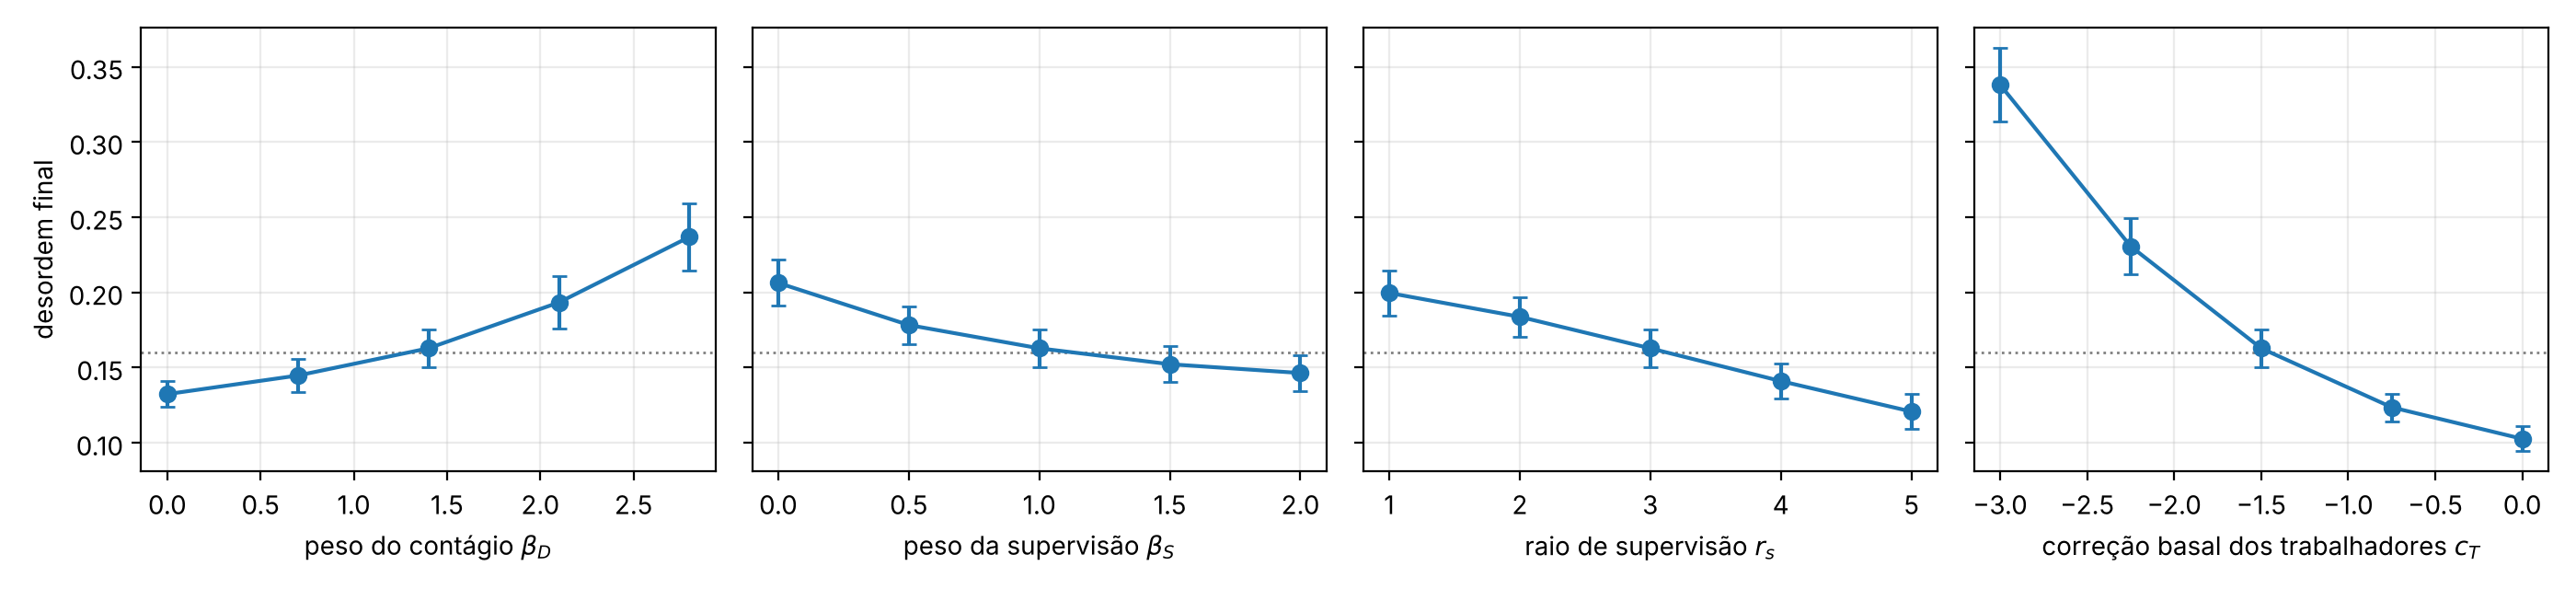
\includegraphics[width=\textwidth]{fig4_sensibilidade.png}
  \caption{Sensibilidade da desordem final a $\beta_D$, $\beta_S$, $r_s$ e $c_T$ (política aleatória; média e IC 95\% de 10 sementes).}
  \label{fig:sens}
\end{figure}

\subsection{Políticas de movimento dos corretores}
A Figura~\ref{fig:politicas} compara as três políticas da Tabela~\ref{tab:politicas} ao variar o número de corretores (esquerda) e o raio de supervisão (direita), com 20 sementes por ponto. No cenário base ($K=8$, $r_s=3$) as três políticas são indistinguíveis: 0,160 (aleatória), 0,155 (reativa) e 0,157 (cobertura), com diferenças de no máximo 0,005 diante de um intervalo de $\pm0{,}011$. A diferença aparece quando a supervisão é ampla. Com $K=16$, a política de cobertura reduz a desordem de 0,124 para 0,097 em relação à aleatória (diferença de $-0{,}027\pm0{,}007$, ou 22\% a menos); com $K=12$, a diferença é $-0{,}016\pm0{,}010$. Com $r_s=5$, a cobertura dá 0,092 contra 0,118 ($-0{,}026\pm0{,}009$), e com $r_s=4$, 0,117 contra 0,139 ($-0{,}022\pm0{,}010$). Em relação ao cenário base, a cobertura com $K=16$ reduz a desordem em 40\% e com $r_s=5$ em 43\%, contra 23\% e 26\% das rotas aleatórias.

Uma estimativa simples explica o padrão. Com posições independentes e uniformes, a fração da grade supervisionada seria $1-(1-49/900)^K$, ou seja, 36\% com $K=8$ e 59\% com $K=16$; o espalhamento sem sobreposição cobriria até 44\% e 87\%. A folga que a cobertura recupera cresce, portanto, de 8 para 28 pontos percentuais, o que é pequeno demais para aparecer com 8 corretores e relevante com 16. A política reativa não melhora o resultado de forma consistente: seu único ganho apreciável ocorre com $r_s=1$ (0,179 contra 0,196, $-0{,}018\pm0{,}012$), e nas demais configurações a diferença para a aleatória é inferior a 0,01, dentro do intervalo de confiança. Uma hipótese compatível com os dados é que, com 16\% das células sujas e espalhadas, o sinal local que guia o corretor reativo é fraco e a desordem não se concentra em pontos que valham perseguir.

\textbf{Conclusão:} a rota dos corretores é uma alavanca secundária e condicional. Mudar a rota de aleatória para cobertura não custa pessoal adicional, mas só traz ganho mensurável (de 0,02 a 0,03 de desordem) quando a supervisão já é ampla ($K\ge12$ ou $r_s\ge4$); perseguir a desordem já instalada (política reativa) não compensa.

\begin{figure}[tbp]
  \centering
  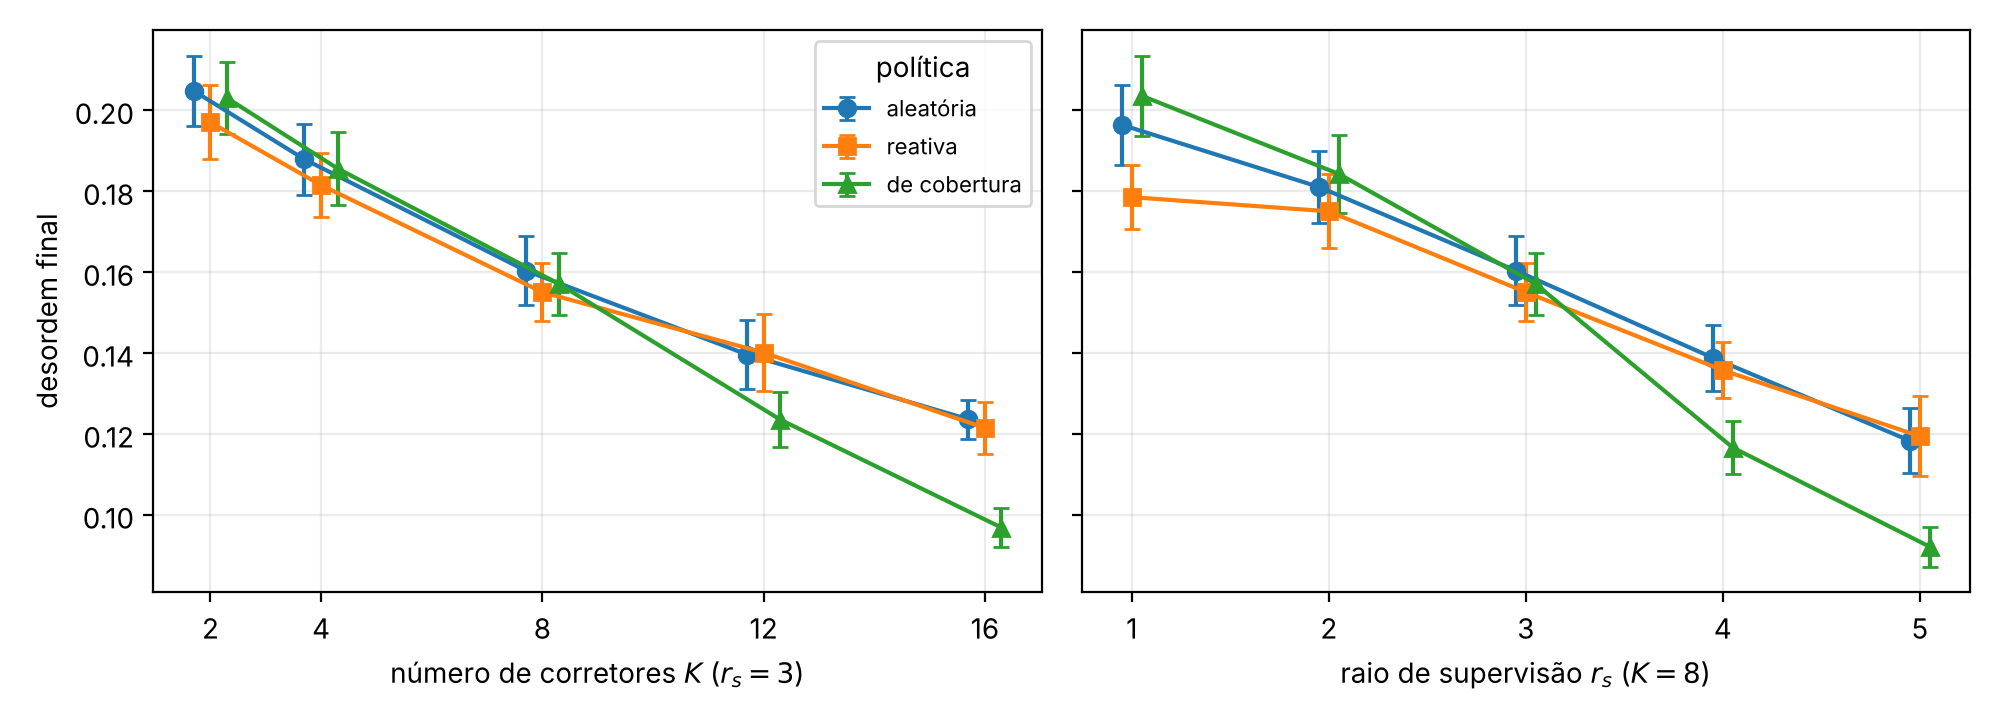
\includegraphics[width=0.9\textwidth]{fig7_politicas.png}
  \caption{Desordem final para as três políticas de movimento em função do número de corretores $K$ (esquerda, $r_s=3$) e do raio de supervisão $r_s$ (direita, $K=8$). Média e IC 95\% de 20 sementes; os pontos de uma mesma abscissa foram deslocados horizontalmente para facilitar a leitura.}
  \label{fig:politicas}
\end{figure}

\subsection{Síntese: quanto cada alavanca reduz a desordem}
A Tabela~\ref{tab:alavancas} compara, a partir do cenário base (0,160, IC 95\% $\pm0{,}009$), o efeito de variar cada alavanca em uma magnitude moderada, com 20 sementes por linha.

\begin{table}[t]
\centering
\footnotesize
\caption{Efeito de variações de cada alavanca sobre a desordem final, em relação ao cenário base (0,160). Alavancas que reduzem a desordem em negrito.}
\label{tab:alavancas}
\begin{tabular}{@{}lcccc@{}}
\toprule
Alavanca & Variação & Desordem & Variação relativa & IC 95\% \\
\midrule
\textbf{Moral média $\bar M$} & 0,50 $\to$ 0,75 & 0,076 & $-52\%$ & $\pm0{,}004$ \\
Moral média $\bar M$ & 0,50 $\to$ 0,25 & 0,328 & $+104\%$ & $\pm0{,}015$ \\
\textbf{Pressão $P$} & 0,50 $\to$ 0,25 & 0,120 & $-25\%$ & $\pm0{,}007$ \\
Pressão $P$ & 0,50 $\to$ 0,75 & 0,213 & $+33\%$ & $\pm0{,}011$ \\
\textbf{Correção basal $c_T$} & $-1{,}5\to-1{,}0$ & 0,132 & $-18\%$ & $\pm0{,}007$ \\
Correção basal $c_T$ & $-1{,}5\to-2{,}0$ & 0,203 & $+26\%$ & $\pm0{,}011$ \\
\textbf{Corretores $K$} & 8 $\to$ 12 & 0,140 & $-13\%$ & $\pm0{,}008$ \\
Corretores $K$ & 8 $\to$ 4 & 0,188 & $+17\%$ & $\pm0{,}009$ \\
\textbf{Raio $r_s$} & 3 $\to$ 4 & 0,139 & $-13\%$ & $\pm0{,}008$ \\
Raio $r_s$ & 3 $\to$ 2 & 0,181 & $+13\%$ & $\pm0{,}009$ \\
\textbf{Corretores $K$, rota de cobertura} & 8 $\to$ 16 & 0,097 & $-40\%$ & $\pm0{,}005$ \\
\textbf{Raio $r_s$, rota de cobertura} & 3 $\to$ 5 & 0,092 & $-43\%$ & $\pm0{,}005$ \\
\bottomrule
\end{tabular}
\end{table}

% =====================================================================
\section{Conclusão}\label{sec:conclusao}
% =====================================================================
No modelo, os desvios não escalam por si só nem desaparecem: a desordem converge para um único patamar (0,160 da área no cenário base), determinado principalmente pela moral da equipe e pela facilidade de corrigir o que foi feito errado, e em segundo plano pela pressão e pela cobertura da supervisão. A escalada para a desordem só ocorre quando o contágio da desordem visível passa de um limiar ($\beta_D$ entre 3 e 5, mais que o dobro do valor base) ou quando a moral é muito baixa (desordem de 0,33 com $\bar M=0{,}25$ e de 0,64 com $\bar M=0$). Picos temporários de pressão elevam os desvios em até 67\%, mas o sistema volta ao patamar anterior em cerca de 45 passos, o que é coerente com as melhoras e pioras temporárias observadas na área. Quanto à rota da supervisão, as três políticas de movimento são equivalentes com 8 corretores e raio 3, e a política de cobertura só se destaca com supervisão ampla, onde reduz a desordem em 0,02 a 0,03 em relação à rota aleatória.

\paragraph{Pontos de alavancagem e recomendações.}
Em ordem decrescente de efeito, com os valores da Tabela~\ref{tab:alavancas}:
\begin{enumerate}
  \item \textbf{Investir na moral:} treinamento, reconhecimento e feedback em campo reduzem o erro e aumentam a correção. Elevar a moral média de 0,50 para 0,75 reduz a desordem em 52\% (de 0,160 para 0,076); é a alavanca de maior efeito.
  \item \textbf{Reduzir a pressão operacional:} baixar $P$ de 0,50 para 0,25 reduz a desordem em 25\% (para 0,120), e evitar medidas que aumentem a pressão (laço R2) previne aumentos de até 33\% (para 0,213 com $P=0{,}75$).
  \item \textbf{Facilitar a correção e o descarte correto:} coletores próximos, identificação clara de cada resíduo e limpeza rápida elevam $c_T$ e atacam a sobrecarga cognitiva (causa-raiz 2). Subir $c_T$ de $-1{,}5$ para $-1{,}0$ (a probabilidade de correção do trabalhador médio passa de 50\% para 62\%) reduz a desordem em 18\%.
  \item \textbf{Ampliar a supervisão e adotar a rota de cobertura:} passar de 8 para 12 corretores reduz a desordem em 13\% e de 8 para 16 em 23\%; ampliar o raio de 3 para 4 células reduz 13\% e para 5 células 26\%. Com a rota de cobertura, os ganhos sobem para 40\% (16 corretores) e 43\% (raio 5).
  \item \textbf{Manter o contágio abaixo do limiar:} não deixar desordem visível acumular evita que a norma colapse; com $\beta_D\le2{,}8$ a desordem permanece abaixo de 0,24, enquanto com $\beta_D=5$ chega a 0,74.
\end{enumerate}

\paragraph{Limitações.}
Os parâmetros vêm da literatura e não foram calibrados com dados da área, de modo que os valores absolutos são ilustrativos e as conclusões valem sobretudo como comparações relativas. Pressão e moral são constantes em cada execução, de modo que os atrasos e os laços R2, B1, B2 e B3 do DLC não são simulados diretamente. Todo desvio é tratado como descarte incorreto de resíduo comum, sem desvios médios e graves. A grade é homogênea, sem layout da planta, turnos ou rotinas de trabalho, e as varreduras usam de 4 a 20 sementes por ponto, de modo que diferenças menores que cerca de 0,01 não são distinguíveis do ruído.

{\footnotesize
\setlength{\bibsep}{2pt}
\bibliographystyle{plainnat}
\bibliography{referencias}
}

\end{document}